\chapter{Future Work}

\section{Back-propagation of reflected wave}

When the propagation will reach the end of the sequence, a reflected wave will be
propagated back to the beginning of the sequence. As a consequence the two extrema get 
closer to each other to reach the stabilized state. If we take a sequence of $L$ with
$N$ elements, the end of the sequence is reached after $N$ steps. We know the value
of the wavefront when the end of the sequence is reached and just before the back 
propagation. We want to know the value of this wavefront when the back propagation
starts. Using the equations \eqref{eq:1D:normalized} and \eqref{eq:wavefront}
we can compute this value:

\begin{equation}
    \begin{split}
        u(N,N+1) & = u(N,N) + \alpha \left( u(N-1,N) - u(N,N) \right) \\
                 & = (1 - \alpha)u(N,N) + \alpha \times u(N-1,N)\\
                 & = (1 - \alpha)((1-\alpha^N)L+\alpha^NH) + \alpha \times u(N-1,N)
    \end{split}
    \label{eq:backprop}
\end{equation}
%
If $\alpha=1$ then $u(N,N+1)=\alpha \times u(N-1,N)$

\subsubsection{Assumption to verify}

We have the assumption that the back propagation at the end of the sequence is
like a flip of the start of the sequence. The concentration stays the same in the
sequence during the time (property \eqref{eq:associativity}). Before the back propagation
the start of the sequence is $u(-N,N)=H$ with $N$ the size of the $H$ sequence. At time
$N+1$ the back propagation starts and the concentration start to decrease 
($u(-N,N+1)<H$). While this concentration decrease the concentration at the end of the
sequence is increasing ($u(N,N+1)>L$). Our assumption is that the decreasing concentration
of the start of the sequence is the same as the increasing concentration of the end of the
sequence.


\section{Absorption of \texorpdfstring{$\mathrm{CO_2}$}{CO2} by the cells}

According to the article \cite{Aalto2002}, the $\mathrm{CO_2}$ flux in the leaf cells 
is influenced by several factors:

\begin{itemize}
    \item Light
    \item Temperature
    \item Ambient $\mathrm{CO_2}$ concentration
    \item Photosynthetic capacity of the mesophyll cells
    \item Size of the stoma opening
    \item Leaf structure
    \item Diffusion coefficients in the different parts
\end{itemize}

The $\mathrm{CO_2}$ concentration distribution is a continous sink and relatively constant 
over the airspace, but decrease rapidly in the mesophyll cells. Concentration inside the 
cells did not decrease more than 18\% from the value in the airspace. The article 
\cite{Kaldenhoff2012} says that the $\mathrm{CO_2}$ diffusion can be variable
in short time range, but it's a physical process dependant of structure so the 
diffusion rate is constant for time ranges of hours. This mecanism of $\mathrm{CO_2}$ 
diffusion is a matter of controversy vivid debate in the scientific community.

\subsubsection{Minimal model}

Consider a 1D sequence like on the section \ref{sec:stomata}. We will use the same sequence
of size 100 pixels but this time the end of the sequence will absorb $\mathrm{CO_2}$ and 
the rest of the sequence will diffuse it. We will assume that the diffusion is decrease by 
10\% in the mesophyll cells. In our sequence the ten last pixels will be the mesophyll 
cells. The formula for the diffusion does not change, but the diffusion rate is different. 
Indeed, the diffusion coefficient is different for the mesophyll cells pixels than for the 
rest of the sequence, it's equal to $0.9 \times \alpha$. With this rate of absorption by 
the mesophyll cells, we need $t=10236$ to obtain a concentration of 49\% instead of 
$t=8416$ without absorption. It takes 21\% more time to reach the stabilized state with 
10\% absorption than without absorption.

\subsubsection{Effect of absorption on stabilized concentration}

Because of the absorption phenomena the assumption \eqref{eq:associativity} is not true 
anymore. If the absorption is too high, the concentration will decrease too fast and the 
sequence will not reach the value of 49\%. For the sequence of 100 pixels, when the 
absorption is greater than 16\% the concentration at the end of the sequence will be less 
than 49\%. We want to plot the time taken to reach the value of 49\% at the end of the 
sequence for the different values of the absorption (see \textbf{Figure \ref{fig:absorb}}). We 
can see that the absorption influences a lot the time to reach a state near the stabilized 
state.

\begin{figure}[h]
    \center
    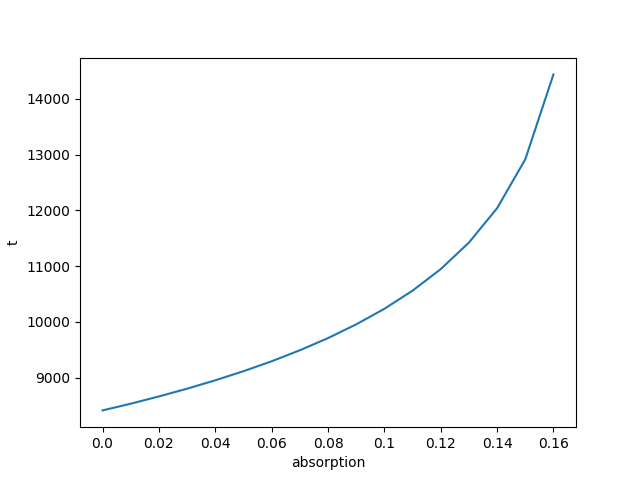
\includegraphics[width=0.66\textwidth]{figures/absorption.png}
    \caption{Time to reach the value of 49\% at the end of the sequence for different values of absorption}
    \label{fig:absorb}
\end{figure}
